\documentclass[12pt, notitlepage]{article}
\usepackage[margin=4cm]{geometry}
\usepackage{hyperref}
\usepackage[english]{babel}
\usepackage{tocloft}
\usepackage{setspace}
\usepackage{graphicx}
\usepackage{caption}
\usepackage{subcaption}
\usepackage{listings}
\usepackage{float}
\usepackage{tabularx}
\usepackage[ruled,vlined]{algorithm2e}
\usepackage[numbers]{natbib}
\usepackage[style=american]{csquotes}
\usepackage{paralist}

\setcounter{tocdepth}{4}
\cftsetindents{paragraph}{1cm}{0cm}


\title{TitlePage}
\author{Stefan Gamerith\\\\
		\emph{Student ID: 0925081}}

\begin{document}
	\maketitle
	\thispagestyle{empty}
	\newpage
\setcounter{page}{1}

\section{Problem Definition}
Knowledge bases handling vast amounts of Linked Data~(e.g. DBpedia~\cite{lehmann2015dbpedia}) are gaining importance, connecting large and distributed datasets. Especially ontology engineering, including ontology creation and ontology evolution, tends to be complex and time-consuming if done by ontology experts.
\citet{wohlgenannt2016crowd}~proposed the uComp Protege plugin for decomposing tasks into simple and small ones, solvable by non-experts. Crowdsourcing methods were used to verify \textit{Relation Correctness~(T2)}, \textit{Relation Type~(T3)} and \textit{Domain Relevance~(T4)}, whereas Term Relatedness~(T1) was not supported. Although evaluation shows that the tool greatly reduces working time by ontology engineers, there were some challenges and limitations. 

This work investigates one such limitation as lacking contextual information in the ontology engineering tasks. More specifically, it investigates what kind of additional context is needed such that the results get more accurate and to what extend it improves the overall workflow. In addition, options for adding task specific contexts, a detailed architecture for an implementation and evaluation against a set of pre-selected ontologies are subjects of contribution. 
\section{Expected Result}
Based on the problem definition above, the following research questions are addressed in this thesis:
\paragraph{RQ1}~\textbf{What are the requirements for an extension of the uComp Protege plugin for adding contextual information to crowdsourcing tasks?}\\
\paragraph{RQ2}~\textbf{What approaches are applicable to facilitate the provision of contextual information for crowdsourcing tasks?}\\
\paragraph{RQ3}~\textbf{Does the proposed extension outperform the existing one on a selected set of ontologies?}\\
This thesis make use of empirical and exploratory approaches strengthening the confidence in answering the research questions. The following results are planned:
\begin{itemize}
	\item Functional and non-functional requirements for building an extension of the uComp Protege plugin.
	\item A detailed study of various options for enhancing crowdsourcing tasks with contextual information.
	\item A designed, implemented and evaluated extension of the uComp Protege plugin.
	\item An in-depth evaluation on the performance of the proposed extension.
	\item A reduction in costs and working time in crowdsourcing tasks while improving quality results from crowds.
\end{itemize}
\section{Methodology and Approach}
The expected results are derived from the following methodology and approach:
\subsection{Literature Research}
For a complete picture on different approaches of how contextual information can be used to improve crowdsourcing tasks, an extensive literature research will be performed. For example one approach from a different research area but also applicable with focus on solving crowdsourcing tasks is ontology matching based on neighboring nodes~\cite{hoffmann2010context}. Although \emph{RQ2} will be addressed directly by this task, literature study is done continuously throughout the whole thesis. 
\subsection{Identify requirements}
Requirements for building an extension of the uComp Protege plugin will be collected by evaluating and extending the requirements of the existing approach~\cite{wohlgenannt2016crowd}. Grouped and evaluated requirements form a basis for choosing the most promising approach for the implementation.
\subsection{Identify different approaches for the implementation}
Based on the insights from literature research, various options for building the extension will be proposed. Each approach will be described in detail, concluding with estimated integration efforts. Based on this estimation, the actual development of the extension will be performed. 
\subsection{Integrate approach in the uComp Protege plugin}
The practical part of this thesis includes extending the uComp Protege plugin to take contextual information into account for performing crowdsourcing tasks. This extension implements all gathered requirements from former requirement analysis. In addition, we will give an overview of the overall plugin architecture as well as the crowdsourcing workflow. 
\subsection{Evaluate performance metrics}
To justify the improvements in a typical ontology engineering setting, a detailed evaluation based on the metrics in~\cite{wohlgenannt2016crowd} will be conducted. More specifically, evaluation metrics include the working time for an ontology engineer, task costs, task duration, data quality and scalability.  

\section{State of the art}
% 1.) Description of current architecture of the uComp Protege Plugin
% 2.) Outline different approaches for adding contextual information to crowdsourcing tasks
%	2.1) Adapt ontology matching techniques by taking neighbouring nodes into account
%	2.2) Adapt Natural language processing techniques (NPL) to discover ambiguities and contradictions
% 3.) Take external information into account or not?
% 4.) Fully automated or guided?
 
 The initial architecture for improving ontology engineering tasks with the help of crowdsourcing that will be used as a baseline for this thesis was introduced by \citet{wohlgenannt2016crowd}. The authors reported that \enquote{its use reduces the working times for the ontology engineers 11 times, lowers the overall task costs by 40\% to 83\% depending on the crowdsourcing settings used and leads to data quality comparable with that of tasks performed by ontology engineers.} The overall workflow ranging from task specification to result interpretation and presentation used by the tool is shown in Figure~\ref{fig:ucomp_workflow}.
\begin{figure}[H]
	 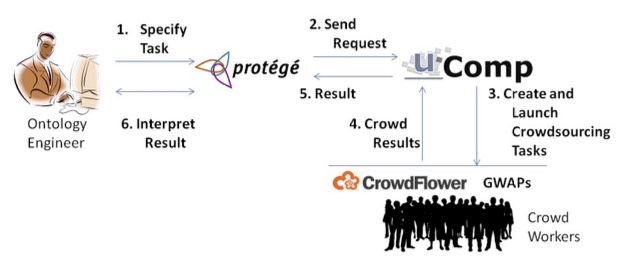
\includegraphics[width=\textwidth]{graphics/ucomp_workflow}
	 \caption{Overall workflow of the uComp Protege Plugin~\cite{wohlgenannt2016crowd}}\label{fig:ucomp_workflow}
\end{figure}

We limit our research to two related approaches described in the next paragraphs. Even though these were applied in different research contexts, applicability can be extended to adding contextual information to crowdsourcing tasks.

An area of interest is ontology matching. \citet{hoffmann2010context} states that \enquote{the context of an ontology can be given by its relations with other ontologies}. Hence, ontology matching is the task of putting ontologies in context whereas content based matching uses its metadata~(e.g. comments, labels, properties, \ldots) to compare ontologies. The context-based matcher Scarlet, first introduced by~\citet{sabou2008scarlet} and extended by~\citet{hoffmann2010context} combines various parameters of context-based matching such as the kind of ontologies that will be used, the method to choose ontologies to anchor concepts, the method to contextualize, the method to aggregate distinct results. 

Another area of interest is Question~Answering~Systems~(QA-Systems). Instead of using a formal query language like SPARQL~\cite{harris2013sparql}, QA-Systems process queries written in natural language. A rather complete overview of QA-Systems in the context of the Semantic Web covering major challenges is given by~\citet{hoffner2016survey}. They identified several challenges such as \emph{Lexical Gap}, \emph{Ambiguity}, \emph{Multilingualism}, \emph{Complex Queries}, \emph{Distributed Knowledge} and \emph{Procedural-,~Temporal-~and~Spatial~Questions}. They concluded that these challenges were subject of active research, leaving room for future improvements. 

\section{Relation to Software Engineering \& Internet Computing}
Researching, evaluating, developing, analyzing and verifying are important skills in the study \emph{Software Engineering \& Internet Computing}, matching the required skillset for answering the research questions in this thesis. Moreover, the development of an extension of the uComp Protege plugin requires an in-depth understanding of all phases of the Software Development Lifecycle, including Requirement~Analysis, Design, Implementation and Maintenance. Furthermore, an overall understanding of scientific principles and approaches as well as advanced knowledge of ontologies and related concepts is necessary. Therefore the qualification profile in the study of \emph{Software Engineering \& Internet Computing} is well covered. 

The following courses in the study of \emph{Software Engineering \& Internet Computing} are relevant:
\begin{itemize}
	\item 183.243 Advanced Software Engineering (PR)
	\item 180.456 Advanced Software Engineering (VO)
	\item 188.399 Introduction to Semantic Web
	\item 188.409 Requirements Engineering and Specification
\end{itemize}

\newpage
\bibliography{literature}
\bibliographystyle{plainnat}

\end{document}